\documentclass{article}
\usepackage{tikz}
\usepackage{geometry}
\usepackage[dvipsnames]{xcolor}
\pagestyle{empty}
\usepackage{luatexja}


\definecolor{CampbellBg}{HTML}{0C0C0C}
\definecolor{CampbellFg}{HTML}{CCCCCC}
\definecolor{CampbellBlack}{HTML}{0C0C0C}
\definecolor{CampbellBlue}{HTML}{0037DA}
\definecolor{CampbellCyan}{HTML}{3A96DD}
\definecolor{CampbellGreen}{HTML}{13A10E}
\definecolor{CampbellPurple}{HTML}{881798}
\definecolor{CampbellRed}{HTML}{C50F1F}
\definecolor{CampbellWhite}{HTML}{CCCCCC}
\definecolor{CampbellYellow}{HTML}{C19C00}
\definecolor{CampbellBrightBlack}{HTML}{767676}
\definecolor{CampbellBrightBlue}{HTML}{3B78FF}
\definecolor{CampbellBrightCyan}{HTML}{61D6D6}
\definecolor{CampbellBrightGreen}{HTML}{16C60C}
\definecolor{CampbellBrightPurple}{HTML}{B4009E}
\definecolor{CampbellBrightRed}{HTML}{E74856}
\definecolor{CampbellBrightWhite}{HTML}{F2F2F2}
\definecolor{CampbellBrightYellow}{HTML}{F9F1A5}

% vi: se ts=2 sw=2 et:


\renewcommand{\kanjifamilydefault}{\gtdefault}
\renewcommand{\familydefault}{\sfdefault}
\newcommand{\docpaperwidth}{21mm}
\newcommand{\docpaperheight}{62mm}

\geometry{
  papersize={\docpaperwidth,\docpaperheight},
  margin=0cm,
  ignoreall=true
}

\usetikzlibrary{backgrounds}
\usetikzlibrary{calc}
\usetikzlibrary{positioning}

\setlength{\parindent}{0cm}
% default color setting
\color{CampbellFg}
\pagecolor{CampbellBg}


\begin{document}
  \center
  % flow - plane
  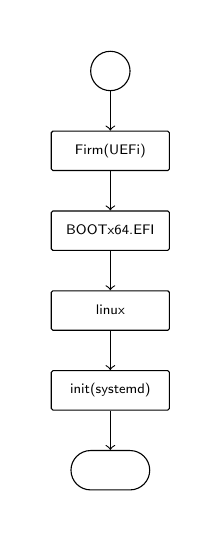
\begin{tikzpicture}[font=\tiny,
    node distance=5mm and 5mm,
    minimum height=5mm,
    minimum width=15mm,
    text height=1mm,
    text depth=0.1mm]
    \node[name=start,shape=circle,minimum size=5mm,draw] {};

    \node[name=firm,
      shape=rectangle,
      rounded corners=0.2mm,
      draw,
      below=of start] {Firm(UEFi)};

    \node[name=bootldr,
      shape=rectangle,
      rounded corners=0.2mm,
      draw,
      below=of firm] {BOOTx64.EFI};

    \node[name=linux,
      shape=rectangle,
      rounded corners=0.2mm,
      draw,
      below=of bootldr] {linux};

    \node[name=init,
      shape=rectangle,
      rounded corners=0.2mm,
      draw,
      below=of linux] {init(systemd)};

    \node[name=end,
      shape=rectangle,
      minimum width=10mm,
      minimum height=5mm,
      rounded corners=2.5mm,
      below=of init,
      draw] {};

    \path (start) edge[->] (firm);
    \path (firm) edge[->] (bootldr);
    \path (bootldr) edge[->] (linux);
    \path (linux) edge[->] (init);
    \path (init) edge[->] (end);


    \path [use as bounding box]
      ($ (start) + (- 15mm / 2 - 3mm, 5mm / 2 + 3mm) $) rectangle
      ($ (end) + (15mm / 2 + 3mm, - 5mm / 2 - 3mm) $);

  \end{tikzpicture}
  \newpage
  % flow - mark firm
  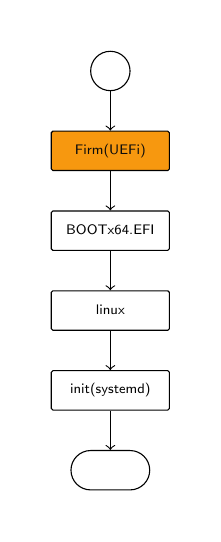
\begin{tikzpicture}[font=\tiny,
    node distance=5mm and 5mm,
    minimum height=5mm,
    minimum width=15mm,
    text height=1mm,
    text depth=0.1mm]
    \node[name=start,shape=circle,minimum size=5mm,draw] {};

    \node[name=firm,
      shape=rectangle,
      rounded corners=0.2mm,
      draw,
      fill=YellowOrange,
      text=CampbellBg,
      below=of start] {Firm(UEFi)};

    \node[name=bootldr,
      shape=rectangle,
      rounded corners=0.2mm,
      draw,
      below=of firm] {BOOTx64.EFI};

    \node[name=linux,
      shape=rectangle,
      rounded corners=0.2mm,
      draw,
      below=of bootldr] {linux};

    \node[name=init,
      shape=rectangle,
      rounded corners=0.2mm,
      draw,
      below=of linux] {init(systemd)};

    \node[name=end,
      shape=rectangle,
      minimum width=10mm,
      minimum height=5mm,
      rounded corners=2.5mm,
      below=of init,
      draw] {};

    \path (start) edge[->] (firm);
    \path (firm) edge[->] (bootldr);
    \path (bootldr) edge[->] (linux);
    \path (linux) edge[->] (init);
    \path (init) edge[->] (end);


    \path [use as bounding box]
      ($ (start) + (- 15mm / 2 - 3mm, 5mm / 2 + 3mm) $) rectangle
      ($ (end) + (15mm / 2 + 3mm, - 5mm / 2 - 3mm) $);
  \end{tikzpicture}
  \newpage
  % flow - mark boot loader
  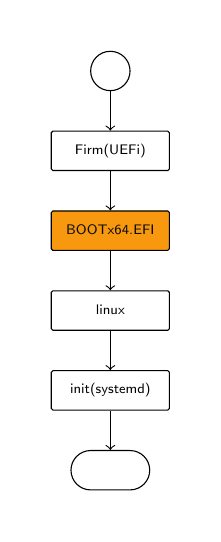
\begin{tikzpicture}[font=\tiny,
    node distance=5mm and 5mm,
    minimum height=5mm,
    minimum width=15mm,
    text height=1mm,
    text depth=0.1mm]
    \node[name=start,shape=circle,minimum size=5mm,draw] {};

    \node[name=firm,
      shape=rectangle,
      rounded corners=0.2mm,
      draw,
      below=of start] {Firm(UEFi)};

    \node[name=bootldr,
      shape=rectangle,
      rounded corners=0.2mm,
      fill=YellowOrange,
      text=CampbellBg,
      draw,
      below=of firm] {BOOTx64.EFI};

    \node[name=linux,
      shape=rectangle,
      rounded corners=0.2mm,
      draw,
      below=of bootldr] {linux};

    \node[name=init,
      shape=rectangle,
      rounded corners=0.2mm,
      draw,
      below=of linux] {init(systemd)};

    \node[name=end,
      shape=rectangle,
      minimum width=10mm,
      minimum height=5mm,
      rounded corners=2.5mm,
      below=of init,
      draw] {};

    \path (start) edge[->] (firm);
    \path (firm) edge[->] (bootldr);
    \path (bootldr) edge[->] (linux);
    \path (linux) edge[->] (init);
    \path (init) edge[->] (end);


    \path [use as bounding box]
      ($ (start) + (- 15mm / 2 - 3mm, 5mm / 2 + 3mm) $) rectangle
      ($ (end) + (15mm / 2 + 3mm, - 5mm / 2 - 3mm) $);
  \end{tikzpicture}
  \newpage
  % flow - mark linux
  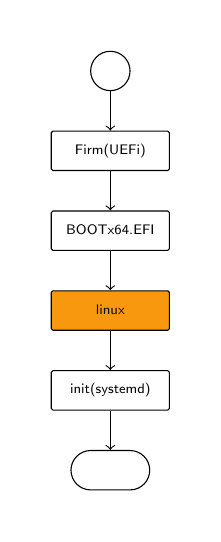
\begin{tikzpicture}[font=\tiny,
    node distance=5mm and 5mm,
    minimum height=5mm,
    minimum width=15mm,
    text height=1mm,
    text depth=0.1mm]
    \node[name=start,shape=circle,minimum size=5mm,draw] {};

    \node[name=firm,
      shape=rectangle,
      rounded corners=0.2mm,
      draw,
      below=of start] {Firm(UEFi)};

    \node[name=bootldr,
      shape=rectangle,
      rounded corners=0.2mm,
      draw,
      below=of firm] {BOOTx64.EFI};

    \node[name=linux,
      shape=rectangle,
      rounded corners=0.2mm,
      fill=YellowOrange,
      text=CampbellBg,
      draw,
      below=of bootldr] {linux};

    \node[name=init,
      shape=rectangle,
      rounded corners=0.2mm,
      draw,
      below=of linux] {init(systemd)};

    \node[name=end,
      shape=rectangle,
      minimum width=10mm,
      minimum height=5mm,
      rounded corners=2.5mm,
      below=of init,
      draw] {};

    \path (start) edge[->] (firm);
    \path (firm) edge[->] (bootldr);
    \path (bootldr) edge[->] (linux);
    \path (linux) edge[->] (init);
    \path (init) edge[->] (end);


    \path [use as bounding box]
      ($ (start) + (- 15mm / 2 - 3mm, 5mm / 2 + 3mm) $) rectangle
      ($ (end) + (15mm / 2 + 3mm, - 5mm / 2 - 3mm) $);
  \end{tikzpicture}
  \newpage
  % flow - mark init
  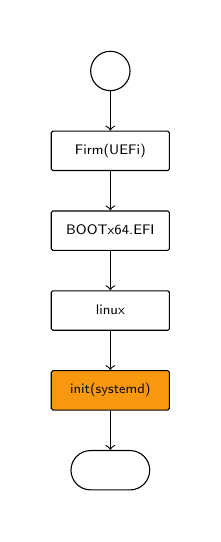
\begin{tikzpicture}[font=\tiny,
    node distance=5mm and 5mm,
    minimum height=5mm,
    minimum width=15mm,
    text height=1mm,
    text depth=0.1mm]
    \node[name=start,shape=circle,minimum size=5mm,draw] {};

    \node[name=firm,
      shape=rectangle,
      rounded corners=0.2mm,
      draw,
      below=of start] {Firm(UEFi)};

    \node[name=bootldr,
      shape=rectangle,
      rounded corners=0.2mm,
      draw,
      below=of firm] {BOOTx64.EFI};

    \node[name=linux,
      shape=rectangle,
      rounded corners=0.2mm,
      draw,
      below=of bootldr] {linux};

    \node[name=init,
      shape=rectangle,
      rounded corners=0.2mm,
      fill=YellowOrange,
      text=CampbellBg,
      draw,
      below=of linux] {init(systemd)};

    \node[name=end,
      shape=rectangle,
      minimum width=10mm,
      minimum height=5mm,
      rounded corners=2.5mm,
      below=of init,
      draw] {};

    \path (start) edge[->] (firm);
    \path (firm) edge[->] (bootldr);
    \path (bootldr) edge[->] (linux);
    \path (linux) edge[->] (init);
    \path (init) edge[->] (end);


    \path [use as bounding box]
      ($ (start) + (- 15mm / 2 - 3mm, 5mm / 2 + 3mm) $) rectangle
      ($ (end) + (15mm / 2 + 3mm, - 5mm / 2 - 3mm) $);
  \end{tikzpicture}
\end{document}
% vi: se ts=2 sw=2 et:
